
While there are methods to determine optimal binning schemes for multi-dimensional datasets with uniform bin widths \parencite{Knuth2019OptimalModels}, no such scheme currently exists for an analysis with non-uniform bin widths. Concordantly, the multidimensional binning in this analysis was heuristically motivated.


In general, bins should be made as small as possible to best approximate a differential cross section, while being large enough to have enough data per bin, and to not be overrun with bin migration issues. In particular, where there was kinematic overlap, the binning scheme for this work was identical to the binning scheme of the CLAS6 result \parencite{Bedlinskiy2014ExclusiveCLAS} to best facilitate data comparisons. Where there was not overlap (at higher values of $x_B$ and $Q^2$), bins were enlarged so as to keep the statistical uncertainty reasonably small. 


The binning region was approximately triangular in $x_B$-$Q^2$ space, and rectangular in $\phi$-t space, and the binning scheme is shown in \figref{fig:databinning}. The $x_B$-$Q^2$ region was bounded on the bottom by the DIS cut $Q^2$ = 1 $GeV^2$, bound on the right by the DIS cut $W^2 > $ 4 $\text{GeV}^2$ ($\frac{Q^2}{x_B}+m_p^2-Q^2>4$), and bound on the left by $p_{e'} > 2 \, \text{GeV/c}$ ($1-\frac{2}{10.604} > 1-\frac{E_{e'}}{E_{beam}} = \frac{Q^2}{2*E_{beam}*x_B*m_p}$). 


    \begin{figure}[H]
        \centering
        
        \subfloat[Inbending $x_B$ vs. $Q^2$]{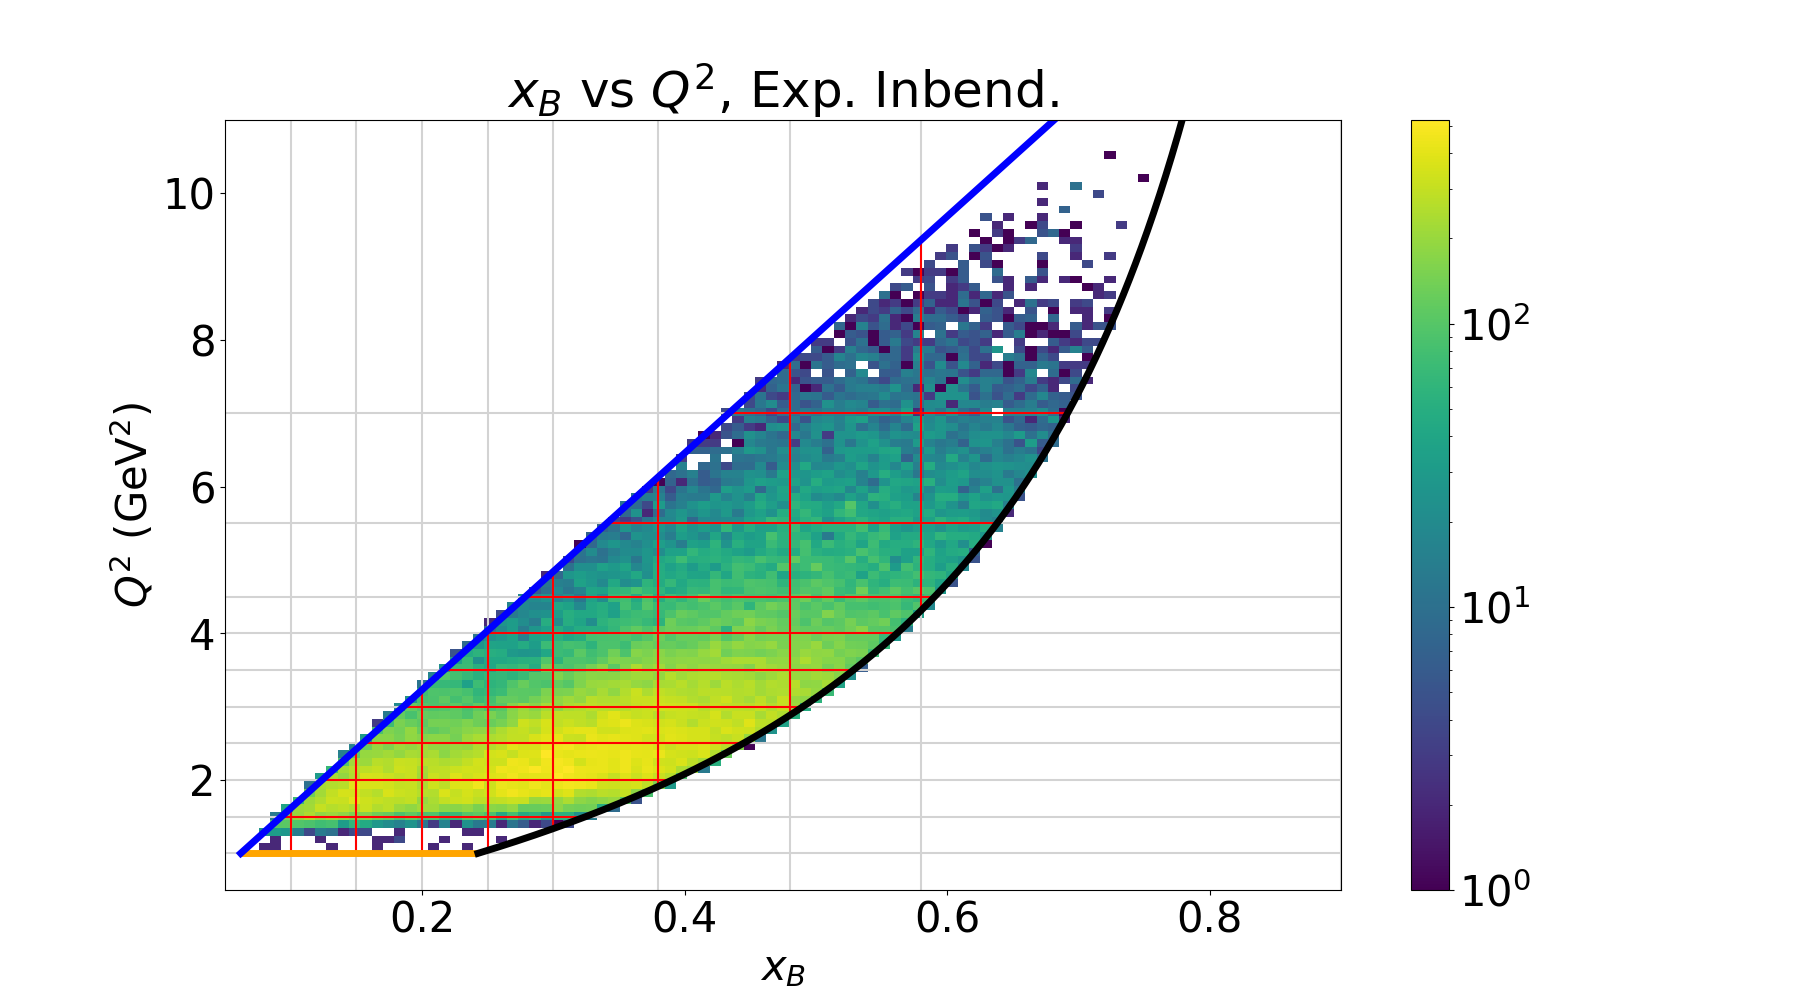
\includegraphics[trim={0 0 5cm 0},clip,width=0.5\textwidth]{Chapters/Ch4-BaseAnalysis/3_Binning/pics/x_B_vs_Q2,_Exp_Inbend.png}}
        \hfill
        \subfloat[Inbending $\phi$ vs. $t$]{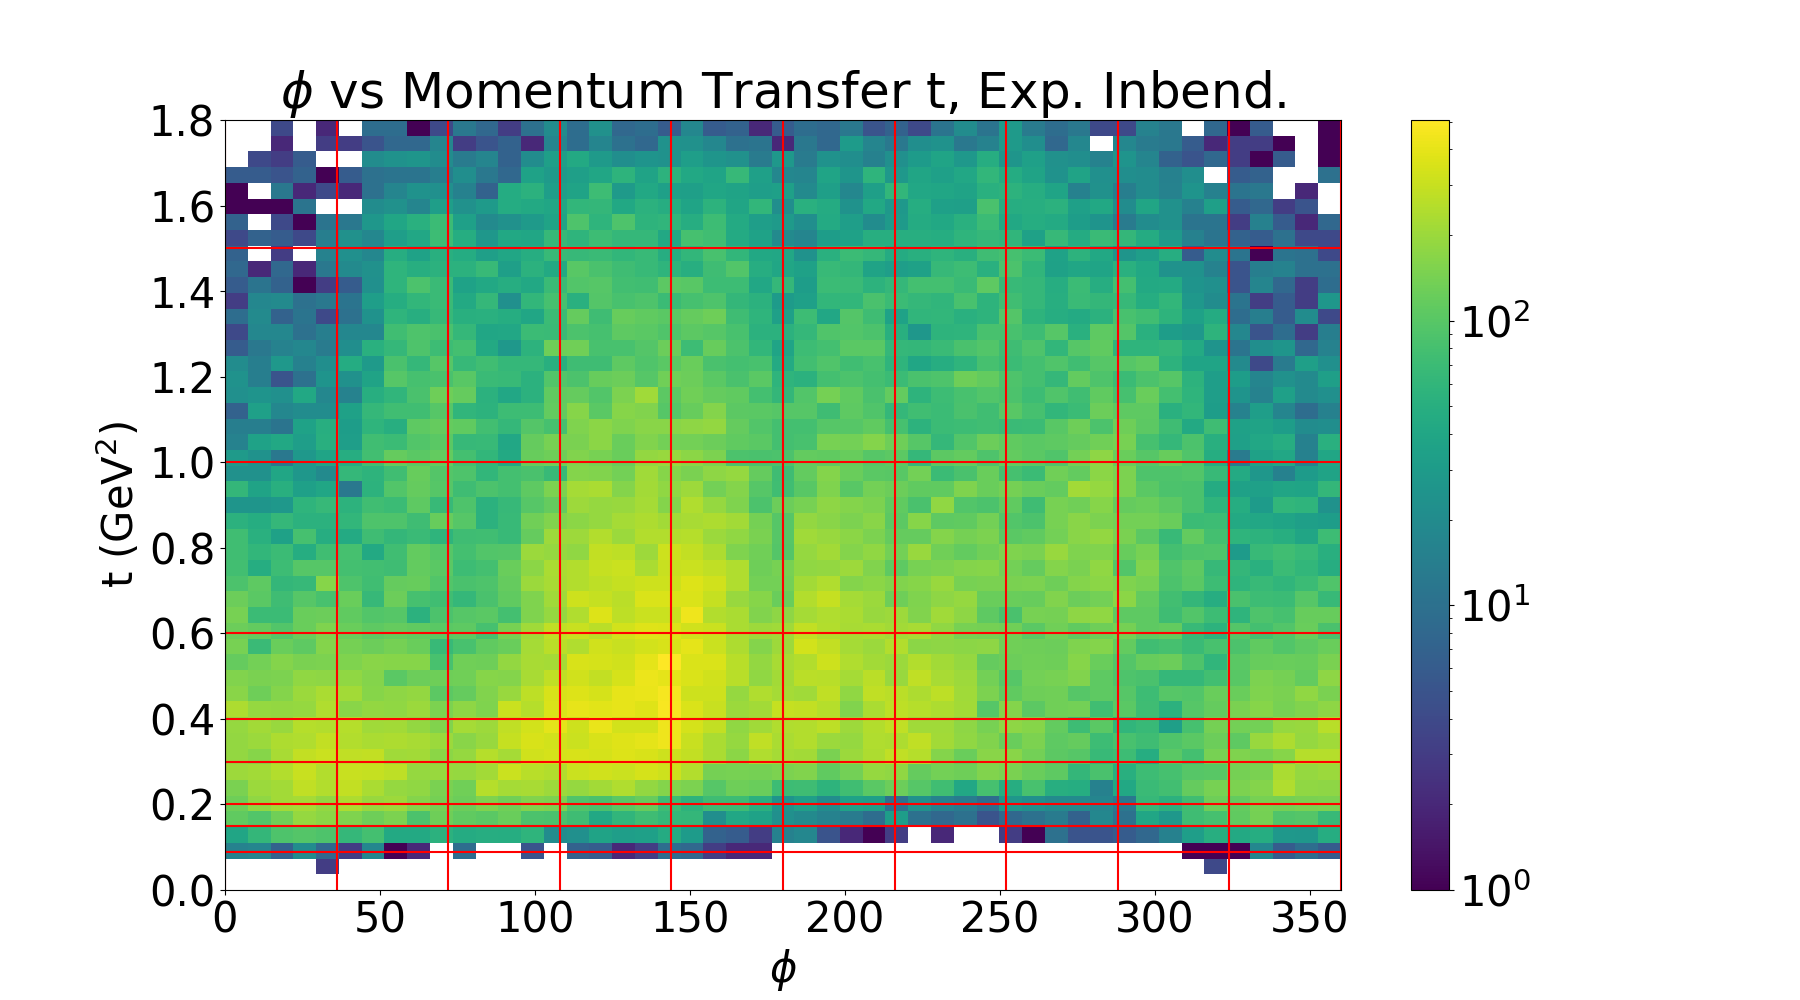
\includegraphics[trim={0 0 5cm 0},clip,width=0.5\textwidth]{Chapters/Ch4-BaseAnalysis/3_Binning/pics/phi_vs_Momentum_Transfer_t,_Exp_Inbend.png}}

        \subfloat[Outbending $x_B$ vs. $Q^2$]{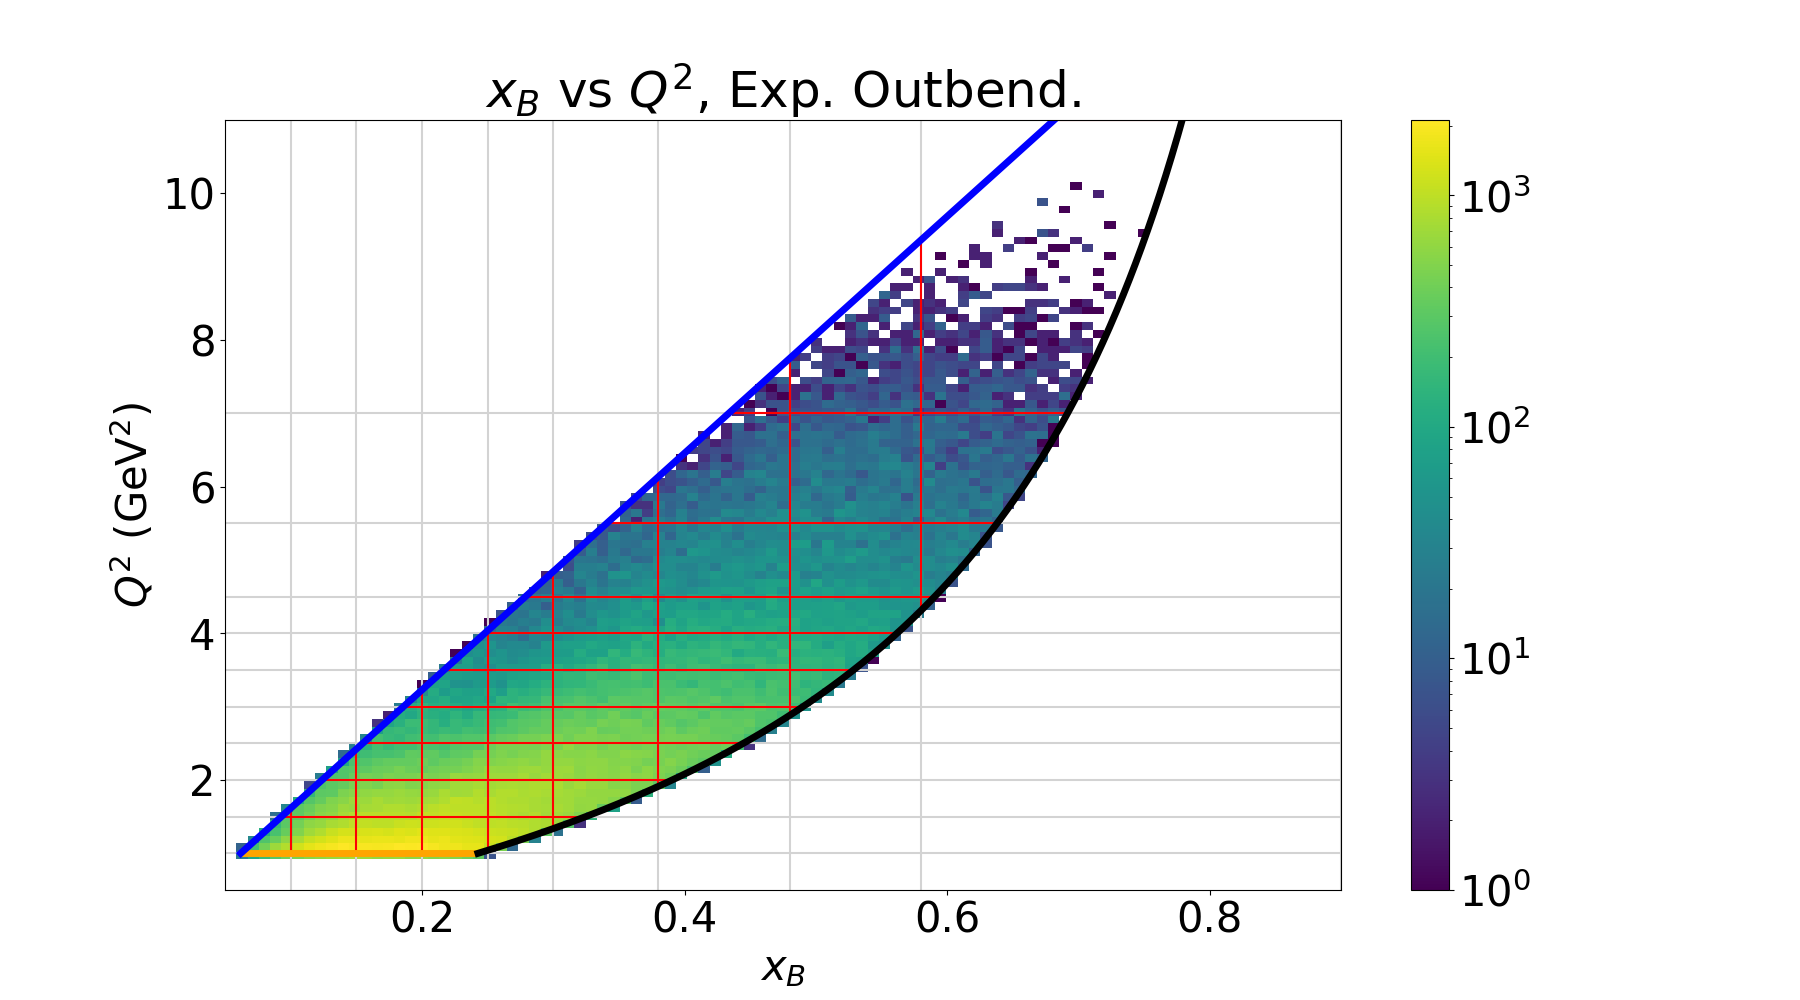
\includegraphics[trim={0 0 5cm 0},clip,width=0.5\textwidth]{Chapters/Ch4-BaseAnalysis/3_Binning/pics/x_B_vs_Q2,_Exp_Outbend.png}}
        \hfill
        \subfloat[Outbending $\phi$ vs. $t$]{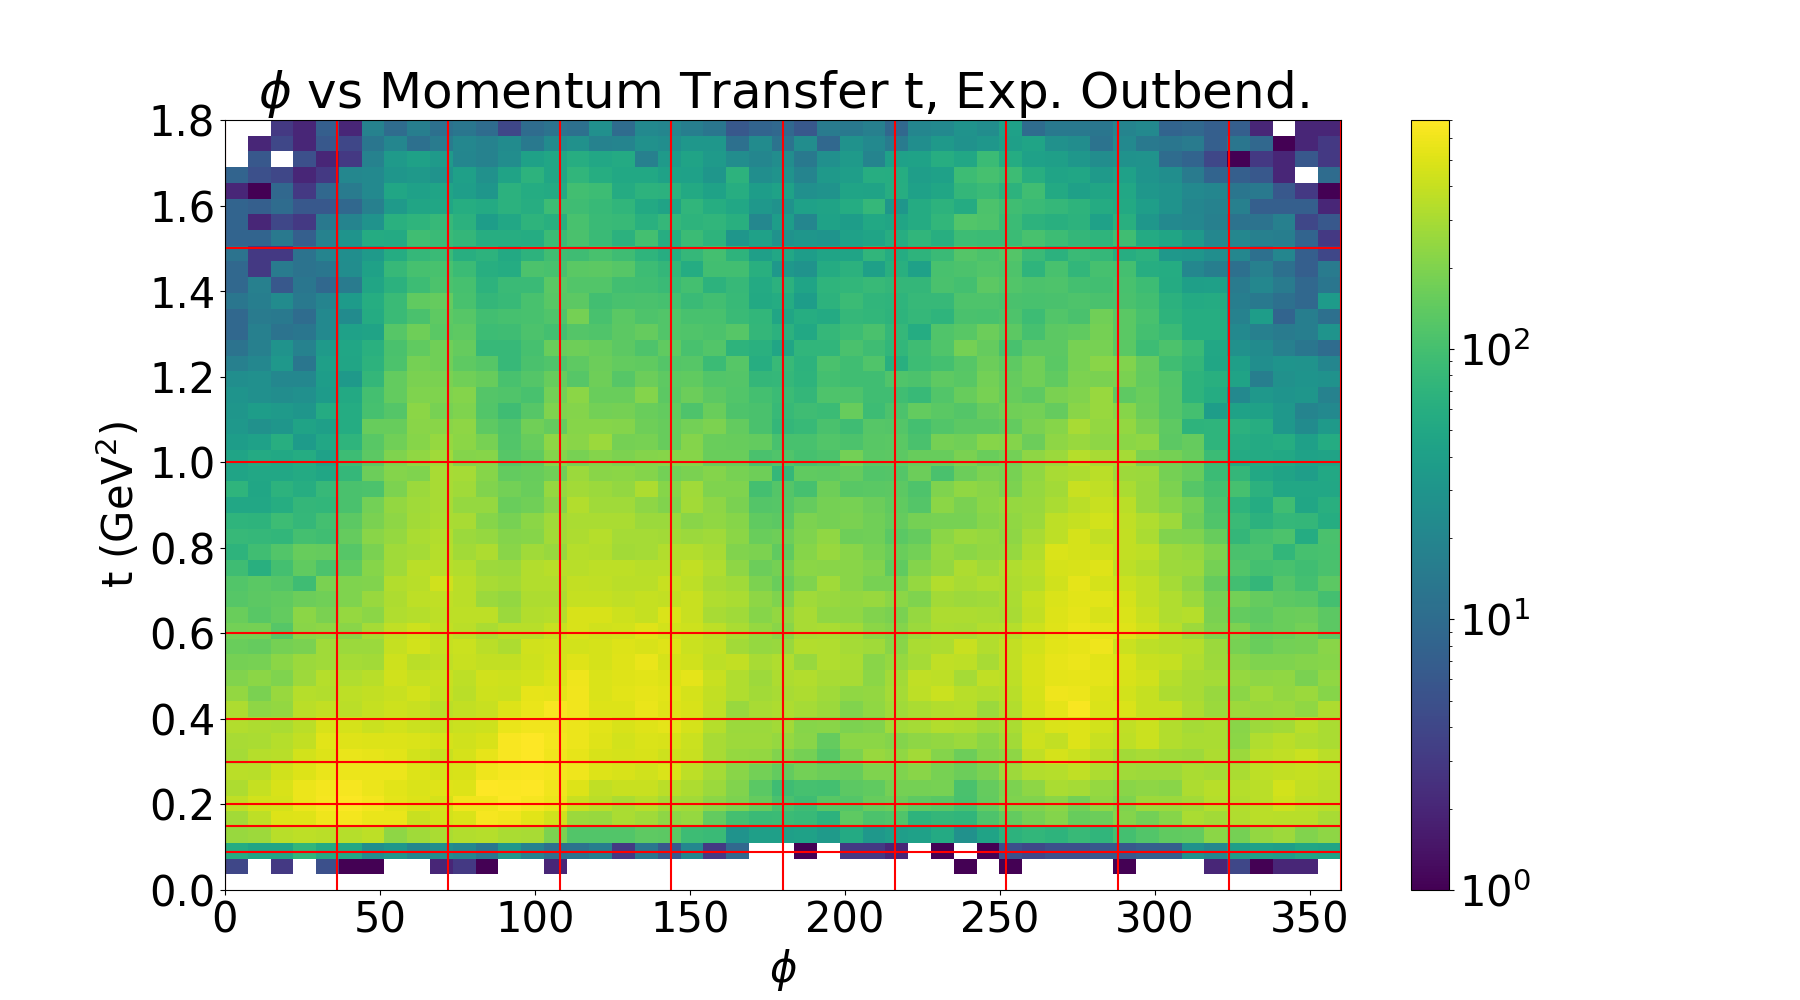
\includegraphics[trim={0 0 5cm 0},clip,width=0.5\textwidth]{Chapters/Ch4-BaseAnalysis/3_Binning/pics/phi_vs_Momentum_Transfer_t,_Exp_Outbend.png}}

        \caption[CLAS12 Data Binning Scheme]{Binning scheme for CLAS12 Fall 2018 Inbending (top row) and Fall 2018 Outbending (bottom row) datasets. Notice the inbending dataset has more sensitivity to higher $Q^2$ data.}\label{fig:databinning}
    \end{figure}






\iffalse
To avoid bin migration, set high q2 on generation.

Figure 5-19: The 2D histograms of events in 2 and  for each configuration of final
level BH-DVCS events. The kinematic regions are bordered by the certain required
conditions: (1)   2 GeV/c (green), (2) 2  1 (GeV/c)2 (blue) and (3)   2
GeV (red).

finite bin effects - center is not average  mean diff

bin volume correction - distribution cutoffs

It is important to choose an optimal multidimensional binning scheme for the cross
section extraction. In this thesis, the bin shape was designed to be a four dimensional
box. Some bins are not well fitted into the box due to the phase space condition. For
example, Fig. 5-19 shows several triangular bins in the 2  plane at the left side,
whose hypotenuse is determined by   2 GeV/c.
The advantage of finer binning is to provide improved density estimation. The
acceptance corrections and the finite bin width effects should increase with the bin
size. However, the bin size cannot be narrower than the effective resolutions in the
binning variables to minimize bin migration. Extremely small bins would not have
any statistical significance in each bin, which would lead to an invalid analysis. It is
important to determine the optimal binning.


The different proton momentum thresholds were considered for the  binning.
The momentum thresholds required for the proton momentum reconstruction, 0.3
GeV/c for CD, 0.42 GeV/c for FD inbending, 0.5 GeV/c for FD outbending lead to
 threhsold of 0.09, 0.17 and 0.23 GeV2 respectively. To consider the bin migration
effect, the  bin was loosely set as [0.110, 0.150, 0.250, 0.400, 0.600, 0.800, 1.000]
GeV2. The number of events in the first bin was estimated with CD protons only.
Likewise, the FD outbending data was not used for the second bin event counting.
There are not enough statistics above t=1 GeV2 to determine the cross sections with
reasonable precision from the RG-A fall 2018 data alone.

The 2 phase space was evenly divided by the bin edges [1.000, 1.200, 1.456,
1.912, 2.510, 3.295, 4.326, 5.761, 7.000] (GeV/c)2 and [0.062, 0.090, 0.118, 0.155,
0.204, 0.268, 0.357, 0.446, 0.581]. The 2   bin boundaries are presented in
2   plane with the 2D histogram of entire experimental data set in Fig. 5-19
with an explanation of the kinematics boundaries at the caption


The  distributions are binned in equal width bins of width 15. Other possible
binning schemes include (1) the adjusted equal width binning to widen the bin width
at the central region to compensate for low statistics, and (2) the equal frequency

binning. The chosen binning scheme has three advantages; (1) the binning scheme is
symmetric with respect to  = 180, (2) the frequency is directly translated into the
probability distribution in the same 2     bin, and (3) it was used by other
experiments [107, 129].

\fi